\chapter{Examples}
\label{cha:examples}


This chapter contains a few another examples from the literature
dealing with chemical reactors. The examples were chosen to
illustrate the ability of the~\fun{dynopt} package to treat the
problems of varying levels of difficulty. The example files can be
found in the directory~\subor{examples/problemX}, where X means the
number of the problem presented in this chapter.

\section{Problem 4}
\label{sec:prob4}

Consider a tubular reactor with  parallel
reactions $A \rightarrow B$, $A \rightarrow C$ taking place
\citep{raj01,dad95,log89} (MATLAB code for this example is located
at \subor{examples/problem4}):
\begin{equation}
\max_{\ve{u}(t)} \mf{J} = x_{2}(t_{f}) \label{eq:tubular}
\end{equation}
such that
\begin{align*}
\dot{x}_1 &=-(u+0.5u^2)x_{1} &x_1(0) &= 1 \\
\dot{x}_2 &=ux_1 &x_2(0) &= 0 \\
u &\in [0,5] & t_f &=1
\end{align*}
where 
\begin{description}
\item $x_{1}(t)$ -- dimensionless concentration of A,
\item $x_{2}(t)$ -- dimensionless concentration of B,
\item $u(t)$ -- control variable.
\end{description}

This problem was treated by~\cite{dad95,log89,raj01} and the value of
performance index of value of 0.57353 was reported as global optimum
by \cite{dad95}. Moreover the value of 0.57284 was reported by
\cite{raj01}. By using 6 collocation points for state variables,
2 collocation points for control variables on the same number of
intervals as in the literature to this problem, we obtained a slightly
closer value of performance index of 0.5734171 to the reported global
maximum (109 iterations, exitflag equal to~1). Ipopt needed more than
11200 iterations and converged to 0.57305461.  
The optimal control
and state profiles are given in Figs. \ref{fig:prob4_u} and
\ref{fig:prob4_x}.

\begin{figure}[htb]
\begin{minipage}[t]{0.5\linewidth}
\centering
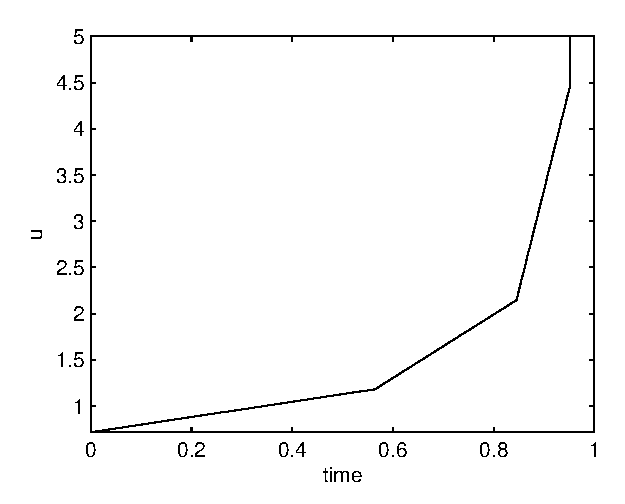
\includegraphics[width=0.9\textwidth]{examples/problem4/graphs/u_624a.eps}
\caption[Problem 4: Control profile]{Control profile for problem 4}
\label{fig:prob4_u}  
\end{minipage}
\begin{minipage}[t]{0.5\linewidth}
\centering
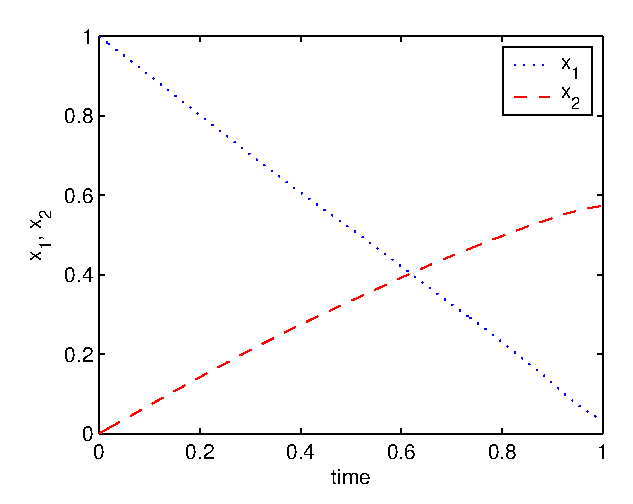
\includegraphics[width=0.9\textwidth]{examples/problem4/graphs/x12_624a.eps}
\caption[Problem 4: State profiles]{State profiles for problem 4}
\label{fig:prob4_x} 
\end{minipage}
\end{figure}
 
\section{Problem 5}
\label{sec:prob5}

Consider a batch reactor~\citep{raj01,dad95} where a series of
reactions $A \rightarrow B\rightarrow C$ is involved. This example is
similar to that in section \ref{sec:brpdae}. The difference is just in
the reactor model description. Here the process is described as an ODE
system (MATLAB code for this example is located at
\subor{examples/problem5}):
\begin{equation}
\max_{\ve{u}(t)} \mf{J} = x_{2}(t_{f}) \label{eq:batch}
\end{equation}
such that
\begin{align*}
\dot{x}_1&=-k_{1}x_{1}^{2} &x_1(0) &= 1 \\
\dot{x}_2&=k_{1}x_{1}^{2}-k_{2}x_{2} &x_2(0) &= 0 \\
k_1 &=4000e^{(-\frac{2500}{T})} &k_2 &=620000e^{(-\frac{5000}{T})} \\
T &\in [298,398] & t_f &=1
\end{align*}
where
\begin{description}
\item $x_{1}(t)$ -- concentration of A,
\item $x_{2}(t)$ -- concentration of B,
\item $T$ -- temperature (control variable).
\end{description}

The objective of problem~\eqref{eq:batch} is to obtain the optimal
temperature profile that maximises the yield of the intermediate
product B at the end of a specified time of operation in a batch
reactor where the reaction $A \rightarrow B \rightarrow C$ take
place. The problem was solved using a relaxed reduced space SQP
strategy by~\cite{log89} and the value of 0.610775 was reported as
global maximum.~\citeauthor{raj01} reached the value of 0.61045. We
obtained optimal value of 0.6107682 (1000 iterations, 11468 function
evaluations, exitflag equal to~0 (maxiter exceeded), by using
5 collocation points for state variables and keeping control variable
profile as piecewise linear on 4 time intervals. This is quite closer
to the global one. The same settings for ipopt resulted in
a non-optimal solution. The optimal control
and state profiles are given in Figs.~\ref{fig:prob5_u} and
\ref{fig:prob5_x}.
  
\begin{figure}[htb]
\begin{minipage}[t]{0.5\linewidth}
\centering
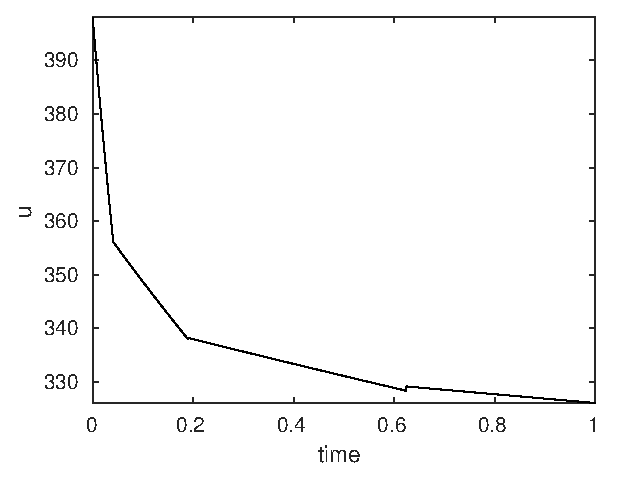
\includegraphics[width=0.9\textwidth]{examples/problem5/graphs/u_524a.eps}
\caption[Problem 5: Control profile]{Control profile for problem 5}
\label{fig:prob5_u}  
\end{minipage}
\begin{minipage}[t]{0.5\linewidth}
\centering
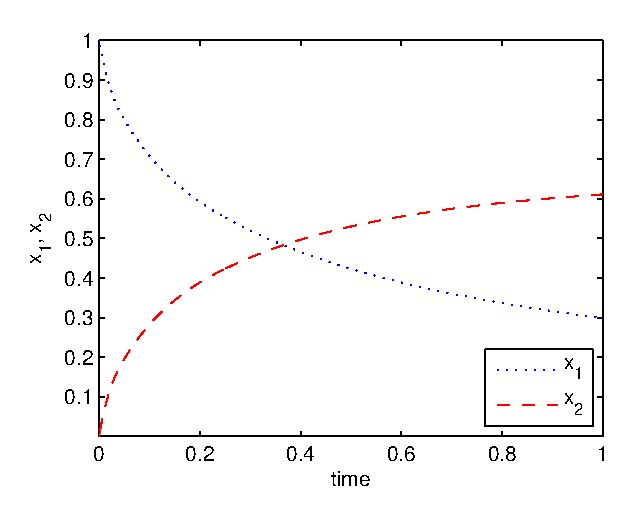
\includegraphics[width=0.9\textwidth]{examples/problem5/graphs/x12_524a.eps}
\caption[Problem 4: State profiles]{State profiles for problem 5}
\label{fig:prob5_x} 
\end{minipage}
\end{figure}

\section{Problem 6}
\label{sec:prob6}

Consider a catalytic plug flow reactor~\citep{raj01,dad95} involving
the following reactions (MATLAB code for this example is located at
\subor{examples/problem6}):\\ 
$A \leftrightarrow B\rightarrow C$
\begin{equation}
\max_{\ve{u}(t)} \mf{J} = 1-x_{1}(t_{f})-x_{2}(t_{f})
\label{eq:plugflow} 
\end{equation}
such that
\begin{align*}
\dot{x}_1&=u(10x_2-x_1) &x_1(0) &= 1 \\
\dot{x}_2&=-u(10x_2-x_1)-(1-u)x_2  &x_2(0) &= 0 \\
u &\in [0,1] & t_f &=12
\end{align*}
where
\begin{description}
\item $x_1(t)$ -- mole fraction of A,
\item $x_2(t)$ -- mole fraction of B,
\item $u(t)$ -- fraction of type 1 catalyst.
\end{description}

Optimisation of this problem has also been analysed. This problem was
solved by~\cite{log89,raj01} and the optima 0.476946, 0.47615 were
reported. Value of the performance index obtained for this problem
using~\fun{dynopt} was 0.477712 (243 iterations, exitflag equal to~1,
fmincon) or 0.47745804 (165 iterations, ipopt). In this case
5 collocation points for state variables and 2 collocation points for
control variables were chosen. The number of time-intervals have been
set to 12. The optimal control and state profiles are given in
Figs.~\ref{fig:prob6_u} and \ref{fig:prob6_x}.

\begin{figure}[htb]
\begin{minipage}[t]{0.5\linewidth}
\centering
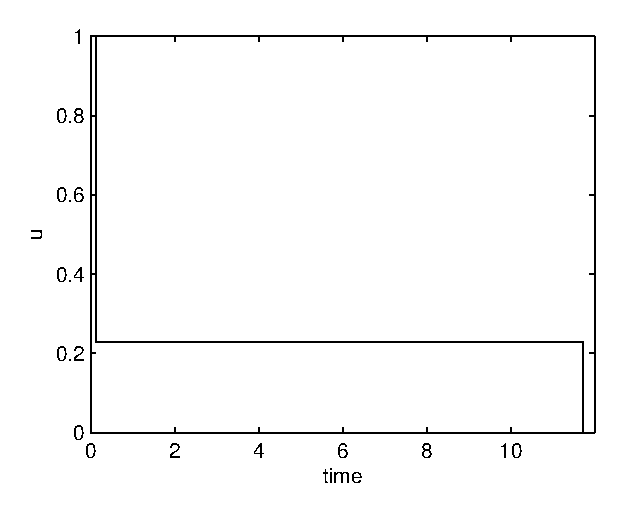
\includegraphics[width=0.9\textwidth]{examples/problem6/graphs/u_5212a.eps}
\caption[Problem 6: Control profile]{Control profile for problem 6}
\label{fig:prob6_u} 
\end{minipage}
\begin{minipage}[t]{0.5\linewidth}
\centering
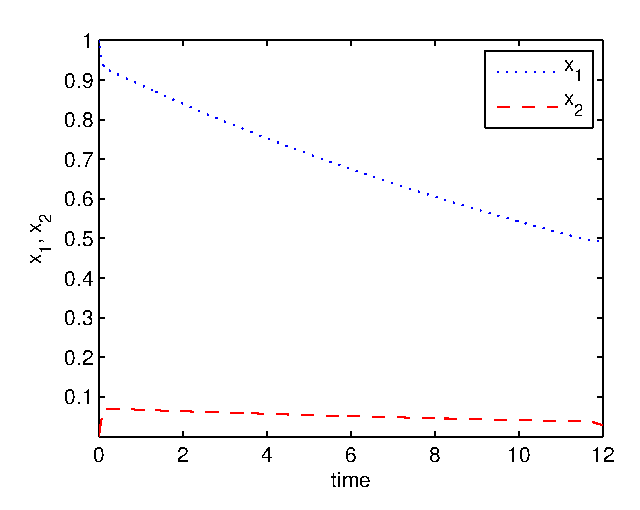
\includegraphics[width=0.9\textwidth]{examples/problem6/graphs/x12_5212a.eps}
\caption[Problem 6: State profiles]{State profiles for problem 6}
\label{fig:prob6_x}  
\end{minipage}
\end{figure}

\section{Problem 7}
\label{sec:prob7}

Consider the following problem~\citep{luu90_52,bal01,fik02} 

\begin{gather}
\max_{\ve{u}(t)} \mf{J} =
\int_{0}^{0.2}\big(5.8(qx_{1}-u_{4})-3.7u_{1}-4.1u_{2}\nonumber\\ % x_{8}\label{eq:e5} 
\mbox{}+q(23x_{4}+11x_{5}+28x_{6}+35x_{7})-5.0u_{3}^{2}\nonumber\\
\mbox{}-0.099\big)\dt \label{eq:cstr}
\end{gather}
such that
\begin{gather*}
\dot{x}_1  =  u_{4}-qx_{1}-17.6x_{1}x_{2}-23x_{1}x_{6}u_{3}\\
\dot{x}_2  =  u_{1}-qx_{2}-17.6x_{1}x_{2}-146x_{2}x_{3}\\
\dot{x}_3  =  u_{2}-qx_{3}-73x_{2}x_{3}\\
\dot{x}_4  =  -qx_{4}+35.2x_{1}x_{2}-51.3x_{4}x_{5}\\
\dot{x}_5  =  -qx_{5}+219x_{2}x_{3}-51.3x_{4}x_{5}\\
\dot{x}_6  =  -qx_{6}+102.6x_{4}x_{5}-23x_{1}x_{6}u_{3}\\
\dot{x}_7  =  -qx_{7}+46x_{1}x_{6}u_{3}\\
% \dot{x}_8  =  5.8(qx_{1}-u_{4})-3.7u_{1}-4.1u_{2}+{}\\
% {}+q(23x_{4}+11x_{5}+28x_{6}+35x_{7})-5.0u_{3}^{2}-0.099\\
\ve{x}(0) = [0.1883~0.2507~0.0467~0.0899~0.1804~0.1394~0.1046]^{\textrm{T}}\\
q = u_{1}+u_{2}+u_{4}\\
0 \leq u_{1} \leq 20\\
0 \leq u_{2} \leq 6\\
0 \leq u_{3} \leq 4\\
0 \leq u_{4} \leq 20\\
t_{f}=0.2
\end{gather*}
where 
\begin{description}
\item $x_{1}(t) - x_{7}(t)$ -- states,
\item $u_{1}(t) - u_{4}(t)$ -- controls.
\end{description}
Analogous to the section \ref{sec:statepathconprob}, the cost function
can be rewritten to the Mayer form by introducing a new state defined
by the integral function with its initial value equal to zero.

This problem was solved by~\cite{fik02,jac69}. Reported optimal value
of 21.757 was obtained using CVP method implemented in DYNO. For this
problem, 4 collocation points for state variables, 2 collocation
points for control variables for 10 intervals were defined and an
optimum was found at value of 21.82346 (840 iterations, exitflag equal
to~1, fmincon). The solver Ipopt did not converge after 10000
iterations. The optimal control and state profiles are given in
Fig.~\ref{fig:prob7}.

\begin{figure}[htb]
\includegraphics[width=0.45\textwidth]{examples/problem7/graphs/u1_4210.eps}
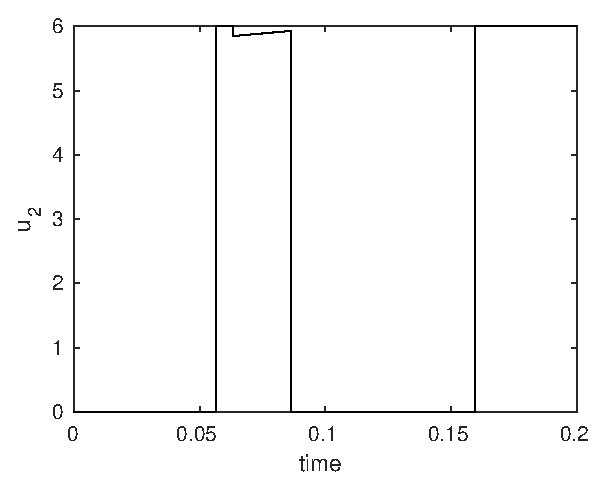
\includegraphics[width=0.45\textwidth]{examples/problem7/graphs/u2_4210.eps}
\includegraphics[width=0.45\textwidth]{examples/problem7/graphs/u3_4210.eps}
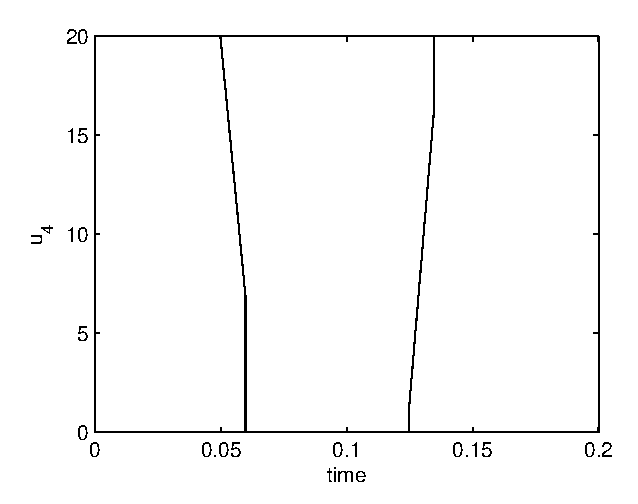
\includegraphics[width=0.45\textwidth]{examples/problem7/graphs/u4_4210.eps}
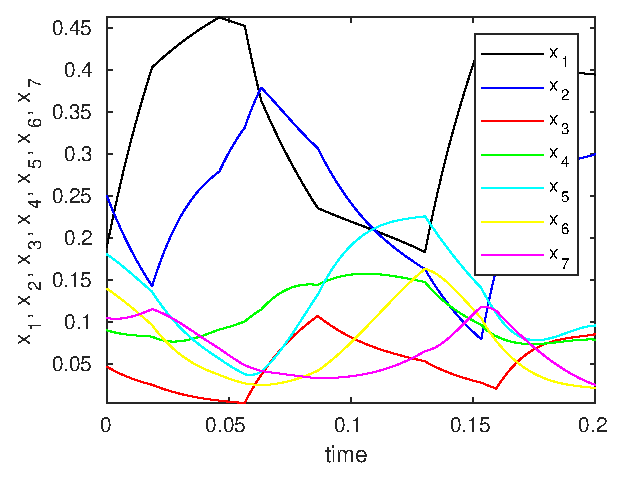
\includegraphics[width=0.45\textwidth]{examples/problem7/graphs/x17_4210.eps}
\caption{Control and state profiles for problem 7} \label{fig:prob7}
\end{figure}


\section{Problem 9}
\label{sec:prob7}

Consider the following problem~\citep{fik10jms} which describes
diafiltration optimal design problem (MATLAB code for this example is located at
\subor{examples/problem9}):
\begin{equation}
  \min_{\alpha(t)} \mf{J} = x_2(t_f)
\end{equation}
subject to differential equations:
\begin{align}
  \dot{x}_1 & = \frac{x_1}{ x_3}
q(x_1, x_2)\left[\mathcal{R}_1(x_1, x_2)-\alpha \right], &
 x_1(0) &= 150  \\
\dot{x}_2 & = \frac{x_2}{ x_3}
q(x_1, x_2)\left[\mathcal{R}_2(x_1, x_2)-\alpha\right], &
 x_2(0) &= 300 \\
\dot{x}_3 &= q(x_1, x_2)(\alpha - 1), &
x_3(0) &= 0.03 
\end{align}
state path constraints:
\begin{align}
  x_3(t) &\ge 0.01 \\
  x_3(t) &\le 0.035
\end{align}
final time constraints:
\begin{align}
  x_3(t_f) &= 0.01 
\end{align}
and simple bound constraints on optimized variable
\begin{align}
  \alpha &\in [0, 1] 
\end{align}
where $\mathcal{R}_1, \mathcal{R}_2, q$ are function of states
determined experimentally as 
\begin{eqnarray} 
q &=& S_1(x_2) e^{S_2(x_2) x_1} \label{eq:Jempiric} \\
\mathcal{R}_1 &=& (z_1 x_2+z_2) x_1  +  ( z_3 x_2+z_4) \label{eq:R1empiric} \\
\mathcal{R}_2 &=& W_1(x_2) e^{W_2(x_2) x_1}	\label{eq:R2empiric}
\end{eqnarray}
where $S_1, S_2, W_1, W_2$ are second order polynomials in $x_2$
\begin{eqnarray} 
S_1(x_2) &=& s_1 x_2^2 + s_2 x_2+s_3 \\
S_2(x_2) &=& s_4 x_2^2 + s_5 x_2+s_6 \\
W_1(x_2) &=& w_1 x_2^2 + w_2 x_2+w_3 \\
W_2(x_2) &=& w_4 x_2^2 + w_5 x_2+w_6 \label{eq:W}
\end{eqnarray}
and $s_{1-6}, z_{1-4},w_{1-6}$ are coefficients that were determined
from laboratory experiments with the process solution
(see Table~\ref{tab:coefficients}).

\begin{table}
  \caption{Experimentally obtained coefficient values for $\mathcal{R}_j$ and $q$.}
  \label{tab:coefficients}
  \centering
  \begin{tabular}{lccc}
    & $s$ & $w$ & $z$ \\ \hline
1  &68.1250\,10$^{-9}$ &7.8407\,10$^{-6}$ &  -0.0769\,10$^{-6}$\\
2  &-56.4512\,10$^{-6}$ &-4.0507\,10$^{-3}$ & -0.0035\,10$^{-3}$ \\
3  & 32.5553\,10$^{-3}$& 1.0585&  0.0349\,10$^{-3}$\\
4  & -4.3529\,10$^{-9}$& 1.2318\,10$^{-9}$& 0.9961 \\
5  & 3.3216\,10$^{-6}$& -9.7660\,10$^{-6}$&  \\
6  & -2.7141\,10$^{-3}$& -1.1677\,10$^{-3}$&  \\
  \end{tabular}
\end{table}

The optimal control profile $\alpha(t)$ is at zero for the first part
of trajectory and one after the switch.  The volume ($x_3$) shows that
the first part of the trajectory basically decreases the volume until
it is on the lower constraint and keeps it approximately constant
until end of the batch. Thus, the optimal control strategy for this
problem represents a traditional diafiltration process with two parts:
pre-concentration followed by approximately constant-volume step until
end of the batch.  The minimum of $x_2(6) = 23.13$ was obtained with
2 piece-wise constant profiles of $\alpha$. Simulation results are
shown in Fig.~\ref{fig:problem-a}.

\begin{figure}[!h]
  \centering
  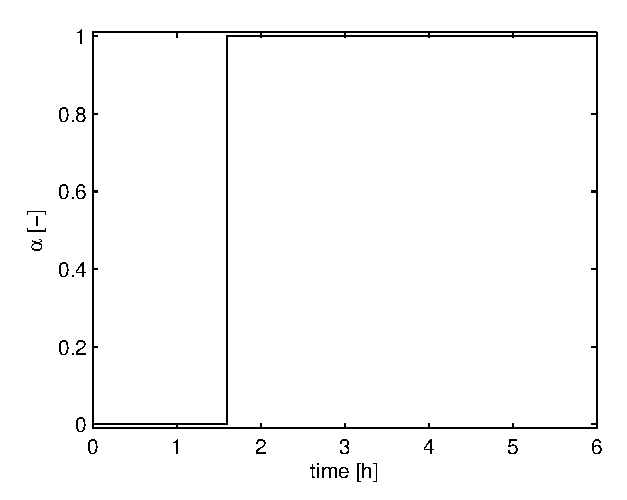
\includegraphics[width=0.32\linewidth]{a-alpha}
  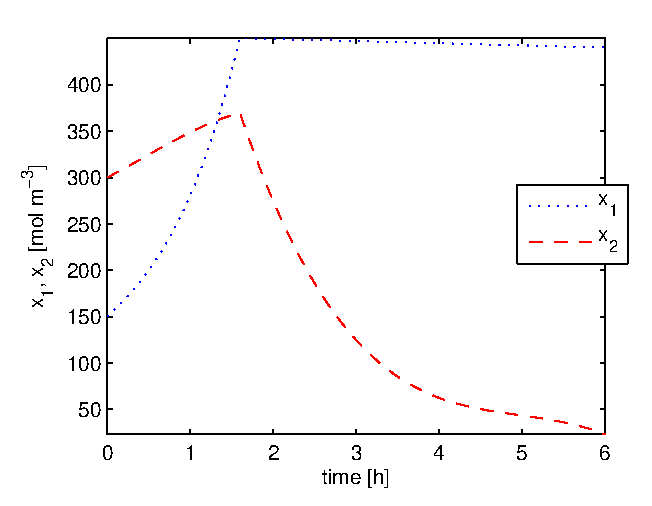
\includegraphics[width=0.32\linewidth]{a-x12} 
  \includegraphics[width=0.32\linewidth]{a-x3}
  \caption{Diafiltration problem: optimal $\alpha$ (left),
    concentrations (middle), and volume (right) as functions of time}
  \label{fig:problem-a}
\end{figure}

%%% Local Variables: 
%%% mode: latex
%%% TeX-master: "dynopt_guide"
%%% End: 
